%*******************************************************************************
%*********************************** First Chapter *****************************
%*******************************************************************************

\chapter{Introduction}  %Title of the First Chapter

\ifpdf
    \graphicspath{{Chapter1/Figs/Raster/}{Chapter1/Figs/PDF/}{Chapter1/Figs/}}
\else
    \graphicspath{{Chapter1/Figs/Vector/}{Chapter1/Figs/}}
\fi

This chapter serves as a rather broad introduction to the topic of this thesis and provides motivation for the work.

\section{General Introduction and Motivation}
Almost any application domain of information systems has some data that is being generated. Data is available in many different forms. One of these forms are data streams. Data streams are not limited to the recent rise in popularity of video and audio streams. On the contrary the application domains that produce data in the form of streams are very diverse. They include for example constantly running business applications that log business activities and events, sensor networks that report usage data or devices that take measurements of physical quantities (such as temperature, pressure, humidity, etc...) at certain points of time. \newline
The fact that streams generate a constant stream of data and thus lead to a constantly growing database is a significant difference to classic applications of data mining in which there is a static (training) database. Despite that significant difference in the data representation, many fields of interest in the context of static databases remain the same for data streams. Common areas of interest are frequent patterns, predictive patterns, association rules, clustering and classification of the data entities. Approaches and algorithms that solve these problems for static databases, while by no means fully researched, are rather well known and evaluated. Applying these methods to data streams can present challenges and may demand many modifications due to the large and possibly infinite amounts of data produced by streams. Naturally, data mining methods for stream data must be especially fast, scalable and memory efficient. \newline
Apart from the additional, algorithmic constraints on memory and computation time, data streams also present conceptual challenges. In contrast to static databases streams may evolve over time, which can make it very difficult for algorithms to assess which past data of the stream should be considered when analyzing the currently incoming data. Recognizing these so called concept drifts is one challenge among many when processing or mining data streams. \newline
A suitable way to look at most data streaming scenarios is that of event streams. An event can be anything that happens in the real world, which can be represented as an element of the stream. These events are commonly referred to as basic or simple events. A frequent area of interest when processing event streams is to mine complex events that consist of multiple basic events with different relationships between each other. Discovering interesting complex event patterns can be tough, especially since there may be a lot of potential candidates. Often we are only interested in specific event combinations. One possible approach to improve the mining process is to use domain knowledge. If the domain knowledge about the underlying event stream contains semantic information about the different event types it is possible to use that knowledge directly in the mining process. Semantic knowledge can take many different forms, a common one being an RDF-graph that can be examined using queries. \newline
Figure \ref{fig_basicProblemStructure} presents the basic idea of semantic complex event mining algorithms. On the lowest level of abstraction we have the low-level event stream, which is the unrefined data coming directly from the sources (for example sensor data). The low-level stream needs to be transformed in some way to an annotated event stream, which then in turn gets mined to discover complex events. The mining algorithm's basic input is the stream of annotated events, but it can also use the previously mentioned semantic knowledge, an ontology, which contains additional information about the event types.
\begin{figure}[h]
	\centering
  	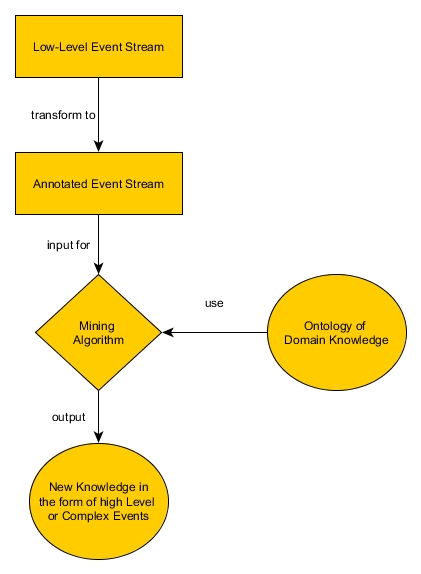
\includegraphics[width=0.5\textwidth]{basicProblemStructure.jpg}
	\caption{General structure of a semantic mining process of complex events}
	\label{fig_basicProblemStructure}
\end{figure}

In terms of the very broad term of complex events this thesis will focus on the subtopic of episode pattern mining from stream data or very large log files or databases. Episodes are a specific kind of complex events and are formally defined in chapter \ref{chapter_related}. For now it is sufficient to know that episodes are essentially complex events in which single events or entire episodes can be combined using two operators: the conjunction and the sequence operator. Figure \ref{fig_simpleEpisodeExample} visualizes a simple episode pattern and example occurrences in a data stream.

\begin{figure}[h]
	\centering
  	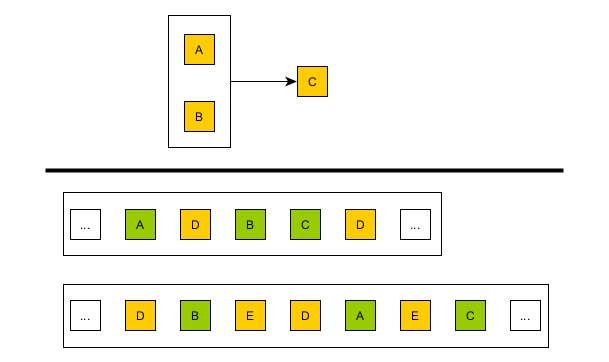
\includegraphics[width=0.5\textwidth]{exampleEpisode.jpg}
	\caption{The top half visualizes an example episode pattern, which consist of a conjunction (A and B must both occur, but the order does not matter) and a sequence (C must occur after A and B). The bottom half shows two windows of an example stream, in which occurrences of the episode are shown in green.}
	\label{fig_simpleEpisodeExample}
\end{figure}

So why is the mining of episodes of interest? There are many real-life use cases in which episode discovery can help predict or prevent problems. The discovery of frequent episodes can for example be related to the discovery of underlying models for data generation, which can help to better understand the data generation process. Another application is to find predictive episodes, meaning episodes which can help to predict events occurring in the future. This has already been applied to predict outages in Finnish power grids (TODO: find a citable source for this). The discovery of predictive episodes is relevant for many domains, for example sensor networks (if a certain chain of events leads to failure, predictive episodes can be used to preemptively expect failures and react accordingly). The domain that will be used in the evaluation of this thesis is stock market prediction. Predicting the overall direction of the stock market or whether individual stocks will rise or fall is a difficult problem that has the obvious application of generating investment strategies. Apart from this, predictive episodes also have use cases in the enforcement of regulations. Predictive episodes could for example be used to detect illegal price arrangements of certain companies, which have been known to happen between oil and gas stations of major companies (TODO: find and cite a source for this). \newline
In contrast to other regression and forecasting methods, such as artificial neural networks, predictive episodes have the advantage that once they are discovered they can make ad-hoc predictions in a fast moving data-stream, whereas neural networks usually forecast the closing values of stock markets of the next day based on the values of previous days. This gives predictive episodes a niche: fast moving (real-time) data-streams that need quick predictions of future events. \newline
The rest of the thesis is outlined as follows: Chapter \ref{chapter_related} gives an overview over relevant related work areas. Chapter \ref{chapter_definitions} explains the basic terminology and gives formal definitions for important terms that are used in this thesis. TODO: the rest of the chapters.
 

%While mining of frequent episodes has already been looked at \cite{frequentEpisodesPHD}, the suggested algorithms use multiple passes over the database to find all frequent episodes. Multiple passes are often not feasible for large data streams, since it is impossible to store the stream in its entire length and thus impossible to look at it more than once. Additionally the state of the art episode definition is rather restrictive in the context of complex events. It is for example impossible to express disjunctions within episodes. Including additional operators like disjunctions would extend the expressive power of episodes, which means that more complex events can be specified and mined as episodes. However, expanding the expressive power also means that frequent episodes will become more difficult to discover, since there are more potential candidates that the algorithm needs to keep track of. This is where the semantic knowledge can come into play. In a realistic scenario, users are not interested in all the frequent complex patterns, since many of them might be meaningless. Semantic or domain knowledge in the form of ontologies can help identify the most interesting candidate patterns and thus help in pruning irrelevant work and therefore improve algorithm performance. For example, one approach could be to only consider the disjunction of events types $A$ and $B$ if we extract knowledge from the ontology that tells us that $A$ and $B$ are similar or belong to the same class of concepts.

%TODO: move the above outcommented part and reuse it?

\section{Contributions and Exact Research Question}
This thesis aims to develop a semantic mining algorithm for predictive episodes. Since the algorithm will be used on data streams, the algorithm must have the following properties:
\begin{itemize}
	\item The Algorithm must have an online learning mode
	\item The Algorithm must be able to adapt to a changing context (as the stream progresses, the underlying model may change completely)
	\item Fast prediction. Since streams, especially in the domain of stock markets, can have a high velocity it is important to be able to quickly predict events. If the prediction takes too long, the event which we want to predict may have already occurred before the algorithm outputs its prediction, thus robbing the user of the opportunity to take precautions.
	\item The Algorithm must not require to store the entire stream of events seen so far, since that is not feasible for most streams.
\end{itemize}

The algorithm will be evaluated on both synthetically generated data and real-life data-sets. The latter ones will be from the domain of stock market prediction, in which the developed algorithm will be empirically compared to other approaches in terms of accuracy measures and execution time.

In summary the research question in particular is:\newline \newline
\textbf{How can event streams be mined for episodes that effectively predict certain event types and how can domain knowledge be used to improve the results or speed of the mining algorithm?}